\documentclass{bioinfo}
\copyrightyear{2005}
\pubyear{2005}

\begin{document}
\firstpage{1}

\title[Application Note]{bioWeb3D a simple online webGL three-dimensional data visualization tool}
\author[Sample \textit{et~al}]{Jean-Baptiste Pettit\,$^{1,*}$ and John Marioni\,$^{1}$\footnote{to whom correspondence should be addressed}}
\address{$^{1}$Department of XXXXXXX, Address XXXX etc.\\
$^{1}$European Bioinformatics Institute}

\history{Received on XXXXX; revised on XXXXX; accepted on XXXXX}

\editor{Associate Editor: XXXXXXX}

\maketitle

\begin{abstract}

\section{Summary:}
An online HTML5/webGL based three dimensional visualization tool has been developed to allow biologists to quickly and simply view interactive and customizable three dimensional representations of their data along with multiple layers of information. Using the Javascript library Three.js, bioWeb3D allows the simultaneous visualization of multiple large datasets through a simple JSON file read and analyzed locally thanks to HTML5 capabilities.

\section{Availability:}
http://ebi.ac.uk/~jbpettit/bioWeb3D

\section{Contact:} \href{jbpettit@ebi.ac.uk}{jbpettit@ebi.ac.uk}
\end{abstract}

\section{Introduction}

Large biological datasets analysis is helped to a great extent by visualization especially when analyzing organized structures. In many fields now, three dimensional datasets are generated along with visualization softwares but never before has a tool allowed biologists to view their research data directly online in an easy, fast, secure and interactive way. Using webGL and HTML 5 three dimensional capabilities and wide range availability, bioWeb3D aims to be a simple non specialized tool for data and information overview.



\section{Technological overview}

bioWeb3D allows the representation of any 3D dataset by defining two file format enabling users to input quickly their own datasets in the application. The format is based on JSON, a widely used structured format on the web. \\
The first file carries the coordinates of all the points in the dataset while the second file describes one or several information layer about the previously defined points. The application allows superposition of different datasets in the same referential.\\
Datasets can be viewed and compared in up to four referential at the same time. What we call information layer represents characteristics attached to the points defined in the dataset or in other words a classification of the data points in different calsses.  Although web based, the application fully written in Javascript doesn’t need to send any data to the host server. To this end the modern browsers local file system reading capabilities are used through the HTML 5 FileReader functionality. This allows the application to handle in a very short time large datasets while remaining entirely safe for the user privacy. \\
It should also be noted that recent browsers improvements regarding GPU acceleration through the webGL paradigm bioWeb3D to visualize several hundred thousand three dimensional data points and to interact with then with a perfect fluidity.\\
Although aimed to remain very simple and easy to use, a few options are available for the user to customize the way their datasets are represented. If the application is used to visualize sequential information such as 3D protein structure, links can be drawn between the points. In the case of living tissue representation, the particles can be left unlinked as individual particles. \\
The way the information layers are shown in the visualization is by coloring the 3D points with regard to which class each point belongs. The user has the option of disabling the view of one or several class within the information layer in order to separately analyze one of the data components. Hidden classes will be shown as the point’s translucent shadow allowing the user to replace the selected information in the global dataset context. Shown classes can be customized in regards to their color separately for each dataset and information layer.\\


\subsection{Defining the input files format}
Within the JSON data-interchange format defined on its official website (http://www.json.org/). This format has been chosen for its rigorous structure allowing fast Javascript objects generation within the browser interpreter. Compared to other data-interchange language such as XML, JSON is also easily human readable thanks to a light-weight syntax.\\
The dataset file root object must be called “dataset”, the object contains :
\begin{itemize}
\item The “name” property of the dataset
\item The “points” property which is a two dimensional array representing a list of (x,y,z) vectors defining the points coordinates.
\end{itemize}

The information layer file has to have its root element named  “cluster”. Because one information file can define multiple information sets, the structure below “cluster” is a list. Each element of the list is structured as follow :
\begin{itemize}
\item The “name” property (optional)
\item The “numClust” property which indicates the number of different classes the data will be assigned to.
\item The “labels” property which defines a list of names for the “numClust” classes previously defined (optional)
\item The values property which defines the class of each point in the dataset. As points don't have a single ID, this property must be in the same order and have the same length than the points defined in the dataset file.
\end{itemize}
Exact specifications and examples of the file formats can be found online at https://github.com/jibooo/bio3D/wiki/Getting-started.\\
Many biological results are in fact stored as CSV files. Because the application is designed to handle meta information about the data, CSV files are not directly readable. However we provide easy to use Perl scripts designed to quickly generate JSON files from CSV data. You can find those scripts in the GitHub repository.


\begin{figure}[h!]%figure1
\centerline{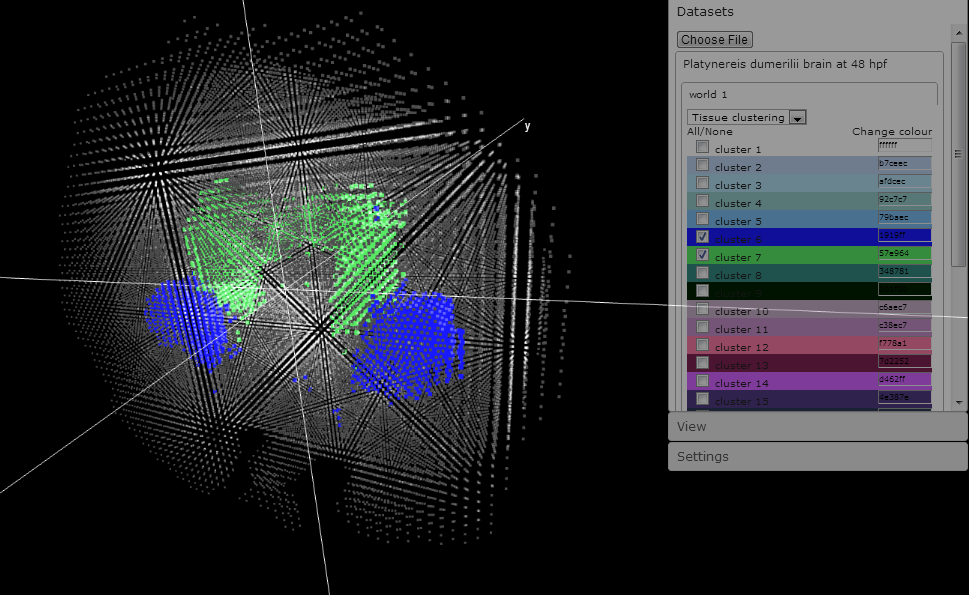
\includegraphics[totalheight=0.2\textheight]{fig1.png}}
\caption{(left) :Marine annelid Platynereis dumerilii single cell clustering results. Two clusters are shown along with the shadow of the remaining cells.(right) : Main carbon chain structure of a Bacterial pentameric ligand-gated ion channel, in red the $\alpha$-helix are highlighted in green the $\beta$-sheets}\label{fig:01}
\end{figure}



\section*{Acknowledgement}
Text Text Text Text Text Text  Text Text.  \citealp{Boffelli03} might want to know about  text text text text

\paragraph{Funding\textcolon} Text Text Text Text Text Text  Text Text.

%\bibliographystyle{natbib}
%\bibliographystyle{achemnat}
%\bibliographystyle{plainnat}
%\bibliographystyle{abbrv}
%\bibliographystyle{bioinformatics}
%
%\bibliographystyle{plain}
%
%\bibliography{Document}


\begin{thebibliography}{}
\bibitem[Bofelli {\it et~al}., 2000]{Boffelli03} Bofelli,F., Name2, Name3 (2003) Article title, {\it Journal Name}, {\bf 199}, 133-154.

\bibitem[Bag {\it et~al}., 2001]{Bag01} Bag,M., Name2, Name3 (2001) Article title, {\it Journal Name}, {\bf 99}, 33-54.

\bibitem[Yoo \textit{et~al}., 2003]{Yoo03}
Yoo,M.S. \textit{et~al}. (2003) Oxidative stress regulated genes
in nigral dopaminergic neurnol cell: correlation with the known
pathology in Parkinson's disease. \textit{Brain Res. Mol. Brain
Res.}, \textbf{110}(Suppl. 1), 76--84.

\bibitem[Lehmann, 1986]{Leh86}
Lehmann,E.L. (1986) Chapter title. \textit{Book Title}. Vol.~1, 2nd edn. Springer-Verlag, New York.

\bibitem[Crenshaw and Jones, 2003]{Cre03}
Crenshaw, B.,III, and Jones, W.B.,Jr (2003) The future of clinical
cancer management: one tumor, one chip. \textit{Bioinformatics},
doi:10.1093/bioinformatics/btn000.

\bibitem[Auhtor \textit{et~al}. (2000)]{Aut00}
Auhtor,A.B. \textit{et~al}. (2000) Chapter title. In Smith, A.C.
(ed.), \textit{Book Title}, 2nd edn. Publisher, Location, Vol. 1, pp.
???--???.

\bibitem[Bardet, 1920]{Bar20}
Bardet, G. (1920) Sur un syndrome d'obesite infantile avec
polydactylie et retinite pigmentaire (contribution a l'etude des
formes cliniques de l'obesite hypophysaire). PhD Thesis, name of
institution, Paris, France.

\end{thebibliography}
\end{document}
